% \documentclass[a4paper,dvipdfmx]{jsarticle}
\RequirePackage{plautopatch}
\documentclass[uplatex,dvipdfmx,a4paper,11pt]{jlreq}

\usepackage{okumacro}
%ルビ用%
\usepackage{indentfirst}
%字下げを保存するための設定 \parでインデント+改行%
\usepackage[dvipdfmx]{graphicx}
\graphicspath{{./assets/}}
\usepackage{float}
%画像挿入パッケージ。graphix=Windows,graphics=Mac%
\usepackage{wrapfig}
%文章を図に回り込ませるパッケージ%
\usepackage{amsfonts}
\usepackage{amssymb}
%数式色々%
\usepackage{bm}
%ベクトル%
\usepackage{url}
%url中の_や\にエラーをはかせないためのパッケージ%
\usepackage{comment}
%複数行コメントのためのパッケージ%
\usepackage{listings, xcolor, inconsolata}
\usepackage{listings-rust}
% Color
\definecolor{Green}{HTML}{009e73}

% Listings
\lstset{
  language=Rust,
  basicstyle=\ttfamily,
  keywordstyle=\bfseries\color{Green},
  showstringspaces=false,
  frame={tb},
  numbers=left,
  xrightmargin=0zw,
  xleftmargin=2zw,
  columns=[l]{fullflexible},
  % columns=fixed,
  % basewidth=0.5em,
}

%コードのためのパッケージ(英語のみ)%
\usepackage{physics}
%物理関係のパッケージ%
\usepackage{amsmath}
%数学関係のパッケージ%
%定理証明関係のパッケージ%
\usepackage{amsthm}
\usepackage{mathtools}
%amsthm%
\theoremstyle{definition}
\newtheorem{dfn}{Definition}[section]
\newtheorem{prop}[dfn]{Proposition}
\newtheorem{lem}[dfn]{Lemma}
\newtheorem{thm}[dfn]{Theorem}
\newtheorem{cor}[dfn]{Corollary}
\newtheorem{rem}[dfn]{Remark}
\newtheorem{fact}[dfn]{Fact}
\renewcommand{\qedsymbol}{$\blacksquare$}
\usepackage{docmute}
%ファイル分割%
\usepackage[hang,small,bf]{caption}
\usepackage[subrefformat=parens]{subcaption}
\captionsetup{compatibility=false}
%各種設定%
\usepackage{color}
%色付け 使うときは\documentclass[dvipdfmx]を追加すること!%
\usepackage{ascmac}
\usepackage{otf}
%ギリシャ数字%
\usepackage{siunitx}
%SI単位系%
\usepackage{tikz}
%tikz%
%枠付%
\usepackage{ascmac}
\usepackage{fancybox}

\usepackage[top=2cm, bottom=2cm, left=2cm, right=2cm]{geometry}
\usetikzlibrary{intersections, calc, arrows, positioning, arrows.meta,automata}
%tikzlibrary%
\renewcommand{\Re}{\real}
\newcommand{\LR}{\Leftrightarrow}
\newcommand{\ii}{\bm{i}}
\begin{document}
\title{統計力学}
\author{
  学籍番号: 21B00349\\
  氏名: 宇佐見 大希\\
}
\maketitle

\section{構成要素である 1 個の二準位系の統計力学}
絶対温度 $T$ の熱浴に系 $X$ が浸けられている状態として、系 $X$ の Hamilton 演算子 $\hat{h}_X$ の固有状態は $\ket{\varphi_1}$ と $\ket{\varphi_2}$ の 2 つだけであり、$\ket{\varphi_1}$ の固有エネルギーは $E_1$ であり、$\ket{\varphi_2}$ の固有エネルギーは $E_2$ であるとする:
\begin{align}
  \hat{h}_X\ket{\varphi_i} & = E_i\ket{\varphi_i} \qquad (i = 1, 2)。
\end{align}
ただし $0 < E_1 < E_2$ $\beta = 1/k_BT$ とする。

\begin{itembox}[l]{Q 15-1.}
  このとき正準集団にもとづく統計力学を用いて解析を進めなさい。具体的には分配関数 $z(\beta)$, Helmholtz 自由エネルギー $f$, エントロピー $s$, 内部エネルギー $u$, 比熱 $c$ を求めよ。
\end{itembox}

まず分配関数 $z(\beta)$ について定義より次のようになる。
\begin{align}
  z(\beta) & = \sum_{i} e^{-\beta E_i} = e^{-\beta E_1} + e^{-\beta E_2}.
\end{align}
これより Helmholtz 自由エネルギー $f$ は次のようになる。
\begin{align}
  f & = -k_BT\ln z(\beta) = -\frac{1}{\beta}\ln(e^{-\beta E_1} + e^{-\beta E_2}).
\end{align}
Helmholtz 自由エネルギーが求まれば後は熱力学の公式を用いてエントロピー $s$, 内部エネルギー $u$, 比熱 $c$ は次のように求まる。
\begin{align}
  s & = - \qty(\pdv{f}{T})_{V,N} = - \qty(\pdv{f}{\beta}\pdv{\beta}{T})_{V,N} = k_B\beta^2\qty(\pdv{f}{\beta})_{V,N}                                                          \\
    & = k_B\beta^2\qty(\frac{1}{\beta^2}\ln(e^{-\beta E_1} + e^{-\beta E_2}) - \frac{1}{\beta}\frac{-E_1e^{-\beta E_1} - E_2e^{-\beta E_2}}{e^{-\beta E_1} + e^{-\beta E_2}}) \\
    & = k_B\qty(\ln(e^{-\beta E_1} + e^{-\beta E_2}) + \frac{\beta E_1e^{-\beta E_1} + \beta E_2e^{-\beta E_2}}{e^{-\beta E_1} + e^{-\beta E_2}})
\end{align}
\begin{align}
  u & = f + Ts = \frac{E_1e^{-\beta E_1} + E_2e^{-\beta E_2}}{e^{-\beta E_1} + e^{-\beta E_2}}.
\end{align}
\begin{align}
  c & = \pdv{u}{T} = \pdv{u}{\beta}\pdv{\beta}{T} = -k_B\beta^2\pdv{u}{\beta}                                                                                                         \\
    & = -k_B\beta^2\pdv{\beta}\qty(\frac{E_1 + E_2e^{\beta(E_1 - E_2)}}{1 + e^{\beta(E_1 - E_2)}})                                                                                    \\
    & = -k_B\beta^2\frac{E_2(E_1 - E_2)e^{\beta(E_1 - E_2)}(1 + e^{\beta(E_1 - E_2)}) - (E_1 + E_2e^{\beta(E_1 - E_2)})(E_1 - E_2)e^{\beta(E_1 - E_2)}}{(1 + e^{\beta(E_1 - E_2)})^2} \\
    & = k_B\beta^2\frac{(E_2 - E_1)^2e^{\beta(E_1 - E_2)}}{(1 + e^{\beta(E_1 - E_2)})^2}                                                                                              \\
    & = k_B\qty(\frac{\frac{1}{2}\beta(E_2 - E_1)}{\cosh\frac{1}{2}\beta(E_2 - E_1)})^2.
\end{align}
$\Box$
a

\begin{itembox}[l]{Q 15-2.}
  Q 15-1.では Helmholtz 自由エネルギーを計算して、後は熱力学の公式を用いて計算しましたが、今回は正準集団の理論における固有状態の実現確率を与える確率関数 $p_\beta^{正準}(i)\ (i = 1, 2)$ を計算して、内部エネルギー $u$ とエントロピー $s$ を求める。
\end{itembox}

まず確率関数 $p_\beta^{正準}(i)$ は定義より次のようになる。
\begin{align}
  p_\beta^{正準}(i) & = \frac{e^{-\beta E_i}}{z(\beta)}.
\end{align}
内部エネルギー $u$ はエネルギーの平均を取ることで分かる。
\begin{align}
  u & = \sum_i E_ip_\beta^{正準}(i) = \frac{E_1e^{-\beta E_1} + E_2e^{-\beta E_2}}{e^{-\beta E_1} + e^{-\beta E_2}}.
\end{align}
比熱も Q15-1.と同様に求まる。

エントロピー $s$ は Shannon のエントロピーの公式に代入することで求まる。
\begin{align}
  s & = -k_B\sum_{i = 1,2}p_\beta^{正準}(i)\ln p_\beta^{正準}(i)                                                                                       \\
    & = -k_B\sum_{i = 1,2}\frac{e^{-\beta E_i}}{z(\beta)}(- \ln z(\beta) - \beta E_i)                                                              \\
    & = k_B\qty(\ln(e^{-\beta E_1} + e^{-\beta E_2}) + \frac{\beta E_1e^{-\beta E_1} + \beta E_2e^{-\beta E_2}}{e^{-\beta E_1} + e^{-\beta E_2}}).
\end{align}

\begin{itembox}[l]{Q 15-3.}
  低温極限 ($\beta(E_2 - E_1) \gg 1$) において系は固有エネルギーのより小さい固有状態 1 にほぼ確実に実現され、より大きい固有状態 2 に実現されることはほぼないことを説明せよ。
\end{itembox}

低温極限では $F = E - TS$ よりエントロピーを上げるよりエネルギーが低いものを選んだ方がエネルギーが得となる為に固有エネルギーの低い状態に集まる。実際式でも次のように計算できる。

実際式でも次のようになる。
\begin{align}
   & \quad p_\beta^{正準}(i) = \frac{e^{-\beta E_i}}{z(\beta)} = \frac{e^{-\beta (E_i - E_1)}}{1 + e^{-\beta(E_2 - E_1)}} \approx e^{-\beta (E_i - E_1)} \\
   & \begin{cases}
       p_\beta^{正準}(1) \approx 1 \\
       p_\beta^{正準}(2) \approx e^{-\beta (E_2 - E_1)} \ll 1
     \end{cases}
\end{align}

\begin{itembox}[l]{Q 15-4.}
  高温極限 ($\beta(E_2 - E_1) \ll 1$) において系は固有状態 1, 2 にほぼ同じ確率 $1/2$ で実現されることを説明せよ。
\end{itembox}

高温極限では $F = E - TS$ よりエントロピーを増大させるとエネルギーが得となる為に半々となる。実際式でも次のように計算できる。

\begin{align}
   & \quad p_\beta^{正準}(i) = \frac{e^{-\beta E_i}}{z(\beta)} = \frac{e^{-\beta (E_i - E_1)}}{1 + e^{-\beta(E_2 - E_1)}} \approx \frac{e^{-\beta (E_i - E_1)}}{2} \\
   & \begin{dcases}
       p_\beta^{正準}(1) \approx \frac{1}{2} \\
       p_\beta^{正準}(2) \approx \frac{e^{-\beta (E_2 - E_1)}}{2} \approx \frac{1}{2}
     \end{dcases}
\end{align}

\begin{itembox}[l]{Q 15-5.}
  低温の漸近領域 ($\beta(E_2 - E_1) \gg 1$, $\beta E_1 \gg 1$) において解析せよ。
\end{itembox}

$x \to 0$ において $(1 + x)^{-1} \approx 1 - x$ と近似できることを用いて、それぞれの熱力学量は次のように計算できる。
\begin{align}
  z & = e^{-\beta E_1} + e^{-\beta E_2}                                                                                                           \\
    & = e^{-\beta E_1}(1 + e^{-\beta (E_2 - E_1)})                                                                                                \\
    & \approx e^{-\frac{E_1}{k_BT}}                                                                                                               \\
    & \to 0                                                                                                                                       \\
  f & = -\frac{1}{\beta}\ln (e^{-\beta E_1} + e^{-\beta E_2})                                                                                     \\
    & = -\frac{1}{\beta}\ln e^{-\beta E_1}(1 + e^{-\beta (E_2 - E_1)})                                                                            \\
    & \approx E_1 - \frac{1}{\beta}e^{-\beta (E_2 - E_1)}                                                                                         \\
    & \approx E_1 - k_BTe^{-\frac{E_2 - E_1}{k_BT}}                                                                                               \\
    & \to E_1                                                                                                                                     \\
  s & = k_B\qty(\ln(e^{-\beta E_1} + e^{-\beta E_2}) + \frac{\beta E_1e^{-\beta E_1} + \beta E_2e^{-\beta E_2}}{e^{-\beta E_1} + e^{-\beta E_2}}) \\
    & = k_B\qty(\ln e^{-\beta E_1}(1 + e^{-\beta (E_2 - E_1)}) + \frac{\beta E_1 + \beta E_2e^{-\beta (E_2 - E_1)}}{1 + e^{-\beta (E_2 - E_1)}})  \\
    & \approx k_B\qty(-\beta E_1 + e^{-\beta (E_2 - E_1)} + (\beta E_1 + \beta E_2e^{-\beta (E_2 - E_1)})(1 - e^{-\beta (E_2 - E_1)}))            \\
    & \approx k_B \frac{E_2 - E_1}{k_BT}e^{- \frac{E_2 - E_1}{k_BT}}                                                                              \\
    & \to 0                                                                                                                                       \\
  u & = \frac{E_1e^{-\beta E_1} + E_2e^{-\beta E_2}}{e^{-\beta E_1} + e^{-\beta E_2}}                                                             \\
    & = \frac{E_1 + E_2e^{-\beta (E_2 - E_1)}}{1 + e^{-\beta (E_2 - E_1)}}                                                                        \\
    & \approx (E_1 + E_2e^{-\beta (E_2 - E_1)})(1 - e^{-\beta (E_2 - E_1)})                                                                       \\
    & \approx E_1 + (E_2 - E_1)e^{- \frac{E_2 - E_1}{k_BT}}                                                                                       \\
    & \to E_1                                                                                                                                     \\
  c & = k_B\qty(\frac{\frac{1}{2}\beta(E_2 - E_1)}{\cosh\frac{1}{2}\beta(E_2 - E_1)})^2                                                           \\
    & = k_B\qty(\frac{\beta(E_2 - E_1)}{1 + e^{-\beta(E_2 - E_1)}})^2e^{-\beta(E_2 - E_1)}                                                        \\
    & \approx k_B\qty(\frac{E_2 - E_1}{k_BT})^2e^{-\frac{E_2 - E_1}{k_BT}}                                                                        \\
    & \to 0
\end{align}

\begin{itembox}[l]{Q 15-6.}
  高温の漸近領域 ($\beta(E_2 - E_1) \ll 1$, $\beta E_1 \ll 1$) において解析せよ。
\end{itembox}
$x \to 0$ において $e^x \approx 1 + x$ と近似できることを用いて、それぞれの熱力学量は次のように計算できる。
\begin{align}
  z & = e^{-\beta E_1}(1 + e^{-\beta (E_2 - E_1)})                                                                                                                                                                                                                                                 \\
    & \approx (1 - \beta E_1)(2 -\beta (E_2 - E_1))                                                                                                                                                                                                                                                \\
    & \approx 2 - \frac{E_1 + E_2}{k_BT}                                                                                                                                                                                                                                                           \\
    & \to 2                                                                                                                                                                                                                                                                                        \\
  f & = -\frac{1}{\beta}\ln e^{-\frac{1}{2}\beta (E_1 + E_2)}(e^{\frac{1}{2}\beta (E_2 - E_1)} + e^{-\frac{1}{2}\beta (E_2 - E_1)})                                                                                                                                                                \\
    & \approx \frac{1}{2}(E_1 + E_2) - k_BT\ln 2                                                                                                                                                                                                                                                   \\
    & \to -\infty                                                                                                                                                                                                                                                                                  \\
  s & = k_B\qty(\ln e^{-\frac{1}{2}\beta (E_1 + E_2)}(e^{\frac{1}{2}\beta (E_2 - E_1)} + e^{-\frac{1}{2}\beta (E_2 - E_1)}) + \frac{\beta E_1e^{\frac{1}{2}\beta (E_2 - E_1)} + \beta E_2e^{-\frac{1}{2}\beta (E_2 - E_1)}}{e^{\frac{1}{2}\beta (E_2 - E_1)} + e^{-\frac{1}{2}\beta (E_2 - E_1)}}) \\
    & \approx k_B\qty(\ln 2 - \frac{1}{2}\beta (E_1 + E_2) + \frac{\beta}{2}\qty(E_1\qty(1 + \frac{1}{2}\beta (E_2 - E_1)) + E_2\qty(1 - \frac{1}{2}\beta (E_2 - E_1))))                                                                                                                           \\
    & \approx k_B\qty(\ln 2 - \frac{1}{4}\qty(\frac{E_2 - E_1}{k_BT})^2)                                                                                                                                                                                                                           \\
    & \to k_B\ln 2                                                                                                                                                                                                                                                                                 \\
  u & = \frac{E_1e^{\frac{1}{2}\beta (E_2 - E_1)} + E_2e^{-\frac{1}{2}\beta (E_2 - E_1)}}{e^{\frac{1}{2}\beta (E_2 - E_1)} + e^{-\frac{1}{2}\beta (E_2 - E_1)}}                                                                                                                                    \\
    & \approx \frac{1}{2}\qty(E_1\qty(1 + \frac{1}{2}\beta (E_2 - E_1)) + E_2\qty(1 - \frac{1}{2}\beta (E_2 - E_1)))                                                                                                                                                                               \\
    & \approx \frac{1}{2}(E_1 + E_2) - \frac{1}{4}\frac{(E_2 - E_1)^2}{k_BT}                                                                                                                                                                                                                       \\
    & \to \frac{1}{2}(E_1 + E_2)                                                                                                                                                                                                                                                                   \\
  c & = k_B\qty(\frac{\beta(E_2 - E_1)}{e^{\frac{1}{2}\beta(E_2 - E_1)} + e^{-\frac{1}{2}\beta(E_2 - E_1)}})^2                                                                                                                                                                                     \\
    & \approx k_B\frac{1}{4}\qty(\frac{E_2 - E_1}{k_BT})^2                                                                                                                                                                                                                                         \\
    & \to 0
\end{align}

\begin{itembox}[l]{Q 15-7.}
  比熱について解析せよ。
\end{itembox}

まず比熱について次のように定義した関数 $\phi(x)$ を用いて表される。
\begin{align}
  \phi(x) & := \frac{x}{\cosh x}                                                              \\
  c       & = k_B\qty(\frac{\frac{1}{2}\beta(E_2 - E_1)}{\cosh\frac{1}{2}\beta(E_2 - E_1)})^2 \\
          & = k_B\qty(\phi\qty(\frac{1}{2}\beta(E_2 - E_1)))^2
\end{align}
ここで $x\geq 0$ の範囲において $\phi(x)$ が極大となる $x = x_0$ の値を考える。
\begin{align}
       & \left.\dv{\phi}{x}\right|_{x = x_0} = 0          \\
  \iff & \frac{\cosh x_0 - x_0\sinh x_0}{\cosh^2 x_0} = 0 \\
  \iff & x_0\tanh x_0 = 1                                 \\
  \iff & x_0 = 1.199678640257734\ldots
\end{align}

ただしプログラム \ref{newton} を用いて $x\geq 0$ の範囲で $x_0\tanh x_0 = 1$ は $x_0 = 1.199678640257734\ldots$ のとき満たすことが分かる。これより比熱 $c$ は次のように定義される $T_0$ のときに極大を取る。
\begin{align}
   & x_0 = \frac{1}{2}\beta_0(E_2 - E_1) = \frac{1}{2}\frac{E_2 - E_1}{k_BT_0} \\
   & \frac{k_BT_0}{E_2 - E_1} = \frac{1}{2x_0} =  0.41677827980048\ldots
\end{align}

低温、高温で比熱が 0 となる理由は比熱が $C = \dv{E}{T}$ であることより Q15-3, Q15-4 よりエネルギーの確率が極限的に定数となることから比熱は 0 となることが分かる。

\begin{lstlisting}[caption=Newton 法による,label=newton]
fn main() {
    let x0 = newton();
    println!("{}", x0);
    println!("{}", 1.0 / (2.0 * x0));
}

fn newton() -> f64 {
    let mut x = 1.0;
    for _i in 0..5 {
        x = _newton(x);
    }
    x
}

fn _newton(x: f64) -> f64 {
    x - f(x) / _f(x)
}

// f(x) = x tanh x - 1
fn f(x: f64) -> f64 {
    x * x.tanh() - 1.0
}

// f'(x) = x / cosh^2 x + tanh x
fn _f(x: f64) -> f64 {
    x * x.cosh().powi(-2) + x.tanh()
}
\end{lstlisting}

\begin{itembox}[l]{Q 15-8.}
  二準位系の熱力学量のグラフを描け。
\end{itembox}

図 \ref{fig:2level} のように描ける。

\begin{figure}[htbp]
  \begin{center}
    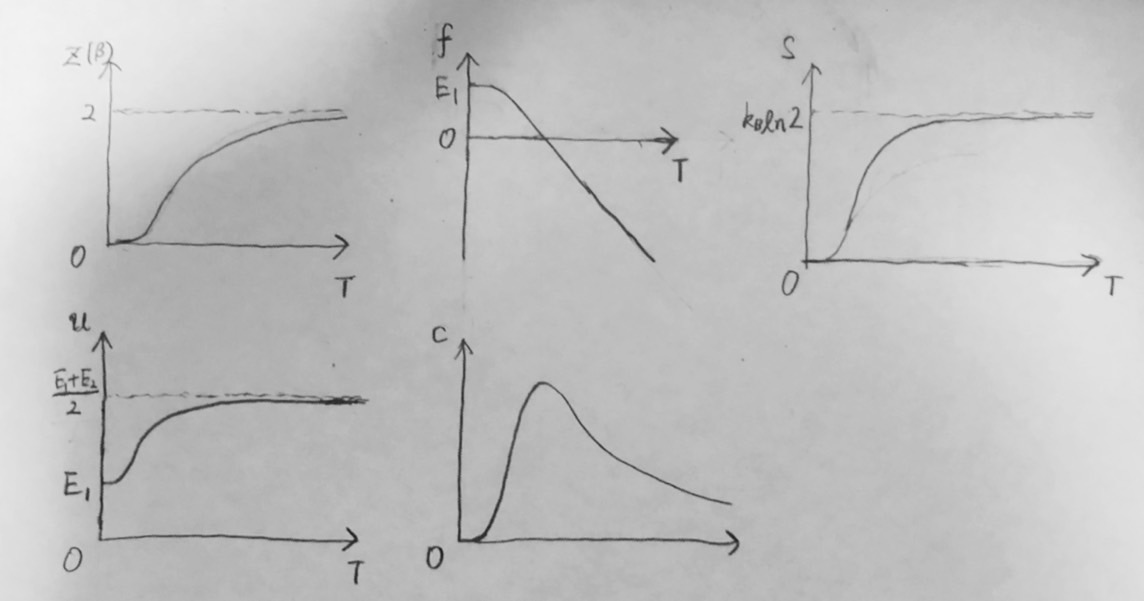
\includegraphics[height=8cm]{2level_system.jpg}
    \caption{二準位系におけるそれぞれの熱力学量の温度 $T$ に関するグラフ}
    \label{fig:2level}
  \end{center}
\end{figure}

\begin{itembox}[l]{Q 15-9.}
  $N$ 個の独立な二準位系からなる系の熱力学量を求めよ。
\end{itembox}

独立な部分系からなる全体系に対する正準集団の理論を用いて次のようになることが分かる。
\begin{align}
  Z(\beta) & = z(\beta)^N = (e^{-\beta E_1} + e^{-\beta E_2})^N                                                                                                \\
  F        & = Nf = -\frac{N}{\beta}\ln(e^{-\beta E_1} + e^{-\beta E_2})                                                                                       \\
  S        & = Ns = Nk_B\qty(\ln(e^{-\beta E_1} + e^{-\beta E_2}) + \frac{\beta E_1e^{-\beta E_1} + \beta E_2e^{-\beta E_2}}{e^{-\beta E_1} + e^{-\beta E_2}}) \\
  U        & = Nu = N\frac{E_1e^{-\beta E_1} + E_2e^{-\beta E_2}}{e^{-\beta E_1} + e^{-\beta E_2}}                                                             \\
  C        & = c = k_B\qty(\frac{\frac{1}{2}\beta(E_2 - E_1)}{\cosh\frac{1}{2}\beta(E_2 - E_1)})^2.
\end{align}

\section{調和振動子の量子力学のまとめ}

1次元の空間を運動する粒子が、次の調和振動子の Hamilton 演算子 $\hat{H}$ に従っているとします:
\begin{align}
  \hat{H} & = \frac{1}{2m}\hat{p}^2 + \frac{1}{2}m\omega^2\hat{q}^2.
\end{align}
ここで、$m$ は粒子の質量であり、$\omega$ は調和振動の角振動数です。また、$\hat{q}$ は粒子の位置座標演算子であり、$\hat{p}$ は運動量演算子です。それらは、次の正準交換関係を満たします:
\begin{align}
  [\hat{q}, \hat{p}] = \hat{q}\hat{p} - \hat{p}\hat{q} = \ii\hbar
\end{align}
ここで、$\hbar$ は Planck 定数です。

この 1 次元調和振動子の固有エネルギー $E_h$ と固有状態 $\ket{n}$ は固有方程式
\begin{align}
  \hat{H}\ket{n} = E_n\ket{n}
\end{align}
を解くことにより定まります。解いた結果は $n = 0, 1, 2, \ldots$ に対して次のとおりです:
\begin{align}
  \begin{dcases}
    E_n        = \qty(n + \frac{1}{2})\hbar\omega \\
    \Psi_n(q) = \braket{q}{n} = \qty(\frac{m\omega}{2^{2n}(n!)^2\pi\hbar})^{\frac{1}{4}}e^{-\frac{m\omega}{2\hbar}q^2}H_n\qty(\sqrt{\frac{m\omega}{\hbar}}q)
  \end{dcases}.
\end{align}
ここで、Hermite 多項式 $H_n(x)$ は次の Rodrigues 公式により定義されます:
\begin{align}
  H_n(x) = (-1)^ne^{x^2}\dv[n]{x}e^{-x^2}.
\end{align}

\section{1 個の調和振動子の統計力学}
\begin{itembox}[l]{Q 16-1.}
  1 個の調和振動子の統計力学における熱力学量を明らかにせよ。
\end{itembox}

熱力学量である分配関数 $z(\beta)$、Helmholtz 自由エネルギー $f$、エントロピー $s$、内部エネルギー $u$、比熱 $c$ について定義や熱力学の公式を用いて次のように求まる。

\begin{align}
  z(\beta) & = \sum_{i = 0}^{\infty}e^{-\beta E_i} = \sum_{i = 0}^{\infty}e^{-\beta\qty(n + \frac{1}{2})\hbar\omega}                                                                                  \\
           & = \frac{e^{-\frac{1}{2}\beta\hbar\omega}}{1 - e^{-\beta\hbar\omega}}                                                                                                                     \\
           & = \frac{1}{2\sinh \frac{1}{2}\beta\hbar\omega}                                                                                                                                           \\
  f        & = -k_BT\ln z(\beta)                                                                                                                                                                      \\
           & = -\frac{1}{\beta}\ln \frac{e^{-\frac{1}{2}\beta\hbar\omega}}{1 - e^{-\beta\hbar\omega}}                                                                                                 \\
           & = -\frac{1}{\beta}\ln \frac{1}{2\sinh \frac{1}{2}\beta\hbar\omega}                                                                                                                       \\
           & = \frac{1}{\beta}\ln(1 - e^{-\beta\hbar\omega}) + \frac{1}{2}\hbar\omega                                                                                                                 \\
           & = \frac{1}{\beta}\ln\qty(2\sinh \frac{1}{2}\beta\hbar\omega)                                                                                                                             \\
  s        & = - \qty(\pdv{f}{T})_{V,N} = k_B\beta^2\qty(\pdv{f}{\beta})_{V,N}                                                                                                                        \\
           & = k_B\beta^2\qty(-\frac{1}{\beta^2}\ln(1 - e^{-\beta\hbar\omega}) + \frac{\hbar\omega}{\beta(1 - e^{-\beta\hbar\omega})})                                                                \\
           & = k_B\beta^2\qty(-\frac{1}{\beta^2}\ln\qty(2\sinh \frac{1}{2}\beta\hbar\omega) + \frac{\frac{1}{2}\hbar\omega\cosh \frac{1}{2}\beta\hbar\omega}{\beta\sinh \frac{1}{2}\beta\hbar\omega}) \\
           & = k_B\qty(-\ln(1 - e^{-\beta\hbar\omega}) + \frac{\beta\hbar\omega}{e^{\beta\hbar\omega} - 1})                                                                                           \\
           & = k_B\qty(-\ln\qty(2\sinh\frac{1}{2}\beta\hbar\omega) + \frac{1}{2}\beta\hbar\omega\coth\frac{1}{2}\beta\hbar\omega)                                                                     \\
\end{align}
\begin{align}
  u & = f + Ts                                                                                                                                                                                      \\
    & = \frac{1}{\beta}\ln(1 - e^{-\beta\hbar\omega}) + \frac{1}{2}\hbar\omega + \frac{1}{\beta}\qty(-\ln(1 - e^{-\beta\hbar\omega}) + \frac{\beta\hbar\omega}{e^{\beta\hbar\omega} - 1})           \\
    & = \frac{1}{\beta}\ln\qty(2\sinh \frac{1}{2}\beta\hbar\omega) + \frac{1}{\beta}\qty(-\ln\qty(2\sinh\frac{1}{2}\beta\hbar\omega) + \frac{1}{2}\beta\hbar\omega\coth\frac{1}{2}\beta\hbar\omega) \\
    & = \qty(\frac{1}{2} + \frac{1}{e^{\beta\hbar\omega} - 1})\hbar\omega                                                                                                                           \\
    & = \frac{1}{2}\hbar\omega\coth\frac{1}{2}\beta\hbar\omega                                                                                                                                      \\
  c & = \pdv{u}{T} = -k_B\beta^2\pdv{u}{\beta}                                                                                                                                                      \\
    & = -k_B\beta^2\qty(-\frac{\hbar\omega e^{\beta\hbar\omega}}{(e^{\beta\hbar\omega} - 1)^2})\hbar\omega                                                                                          \\
    & = k_B\qty(\beta\hbar\omega\frac{e^{\frac{1}{2}\beta\hbar\omega}}{e^{\beta\hbar\omega} - 1})^2                                                                                                 \\
    & = k_B\qty(\frac{\frac{1}{2}\beta\hbar\omega}{\sinh\frac{1}{2}\beta\hbar\omega})^2.
\end{align}

これより求まった。 $\Box$

\begin{itembox}[l]{Q 16-2.}
  低温の漸近領域 ($\beta\hbar\omega \gg 1$) において解析せよ。
\end{itembox}

低温の漸近領域において Q 16-1 の結果は次のように近似できる。ただし、$x\to 0$ のとき $e^x \approx 1 + x$, $(1 + x)^{-1} \approx 1 - x$ と近似できることを用いる。

\begin{align}
  z(\beta) & = \frac{e^{-\frac{1}{2}\beta\hbar\omega}}{1 - e^{-\beta\hbar\omega}}                                       \\
           & \approx e^{-\frac{\hbar\omega}{2k_BT}}                                                                     \\
           & \to 0                                                                                                      \\
  f        & = \frac{1}{\beta}\ln(1 - e^{-\beta\hbar\omega}) + \frac{1}{2}\hbar\omega                                   \\
           & \approx \frac{1}{\beta}(-e^{-\beta\hbar\omega}) + \frac{1}{2}\hbar\omega                                   \\
           & \approx \frac{1}{2}\hbar\omega - k_BTe^{-\frac{\hbar\omega}{k_BT}}                                         \\
           & \to \frac{1}{2}\hbar\omega                                                                                 \\
  s        & = k_B\qty(-\ln(1 - e^{-\beta\hbar\omega}) + \frac{\beta\hbar\omega}{e^{\beta\hbar\omega} - 1})             \\
           & \approx k_B\qty(e^{-\beta\hbar\omega} + \beta\hbar\omega e^{-\beta\hbar\omega}(1 + e^{-\beta\hbar\omega})) \\
           & \approx k_B\frac{\hbar\omega}{k_BT}e^{- \frac{\hbar\omega}{k_BT}}                                          \\
           & \to 0                                                                                                      \\
\end{align}
\begin{align}
  u & = \qty(\frac{1}{2} + \frac{1}{e^{\beta\hbar\omega} - 1})\hbar\omega                              \\
    & \approx \qty(\frac{1}{2} + e^{-\beta\hbar\omega}(1 + e^{-\beta\hbar\omega}))\hbar\omega          \\
    & \approx \frac{1}{2}\hbar\omega + e^{-\beta\hbar\omega}\hbar\omega                                \\
    & \to \frac{1}{2}\hbar\omega                                                                       \\
  c & = k_B\qty(\beta\hbar\omega\frac{e^{\frac{1}{2}\beta\hbar\omega}}{e^{\beta\hbar\omega} - 1})^2    \\
    & \approx k_B\qty(\beta\hbar\omega(e^{-\frac{1}{2}\beta\hbar\omega})(1 + e^{-\beta\hbar\omega}))^2 \\
    & \approx k_B\qty(\frac{\hbar\omega}{k_BT})^2e^{-\frac{\hbar\omega}{k_BT}}                         \\
    & \to 0
\end{align}

\begin{itembox}[l]{Q 16-3.}
  高温の漸近領域 ($\beta\hbar\omega \ll 1$) において解析せよ。
\end{itembox}

高温の漸近領域において Q 16-1 の結果は次のように近似できる。ただし、$x\to 0$ のとき $\ln(1 + x) \approx x$ と近似できることとテイラー展開を用いる。

\begin{align}
  z(\beta) & = \frac{e^{-\frac{1}{2}\beta\hbar\omega}}{1 - e^{-\beta\hbar\omega}}                                                             \\
           & \approx \frac{1 - \frac{1}{2}\beta\hbar\omega}{\beta\hbar\omega}                                                                 \\
           & \approx \frac{k_BT}{\hbar\omega} - \frac{1}{2}                                                                                   \\
           & \to +\infty                                                                                                                      \\
  f        & = \frac{1}{\beta}\ln(1 - e^{-\beta\hbar\omega}) + \frac{1}{2}\hbar\omega                                                         \\
           & \approx \frac{1}{\beta}\qty(\ln \beta\hbar\omega + \frac{1}{2}\beta\hbar\omega)                                                  \\
           & \approx -k_BT\ln\frac{k_BT}{\hbar\omega}                                                                                         \\
           & \to - \infty                                                                                                                     \\
  s        & = k_B\qty(-\ln(1 - e^{-\beta\hbar\omega}) + \frac{\beta\hbar\omega}{e^{\beta\hbar\omega} - 1})                                   \\
           & \approx k_B\qty(-\ln\beta\hbar\omega + 1)                                                                                        \\
           & \approx k_B\ln\frac{k_BT}{\hbar\omega}                                                                                           \\
           & \to +\infty                                                                                                                      \\
  u        & = \frac{1}{2}\hbar\omega\coth\frac{\beta\hbar\omega}{2}                                                                          \\
           & \approx \frac{1}{2}\hbar\omega\qty(\qty(\frac{\beta\hbar\omega}{2})^{-1} + \frac{1}{3}\qty(\frac{\beta\hbar\omega}{2}) + \cdots) \\
           & = k_BT\qty(1 + \frac{1}{12}\qty(\frac{\hbar\omega}{k_BT})^{2} + \cdots)                                                          \\
           & \to +\infty                                                                                                                      \\
\end{align}
\begin{align}
  c & = k_B\qty(\frac{\frac{1}{2}\beta\hbar\omega}{\sinh\frac{1}{2}\beta\hbar\omega})^2                                                               \\
    & \approx k_B\qty(\frac{\beta\hbar\omega}{2}\qty(\qty(\frac{\beta\hbar\omega}{2})^{-1} - \frac{1}{6}\qty(\frac{\beta\hbar\omega}{2}) + \cdots))^2 \\
    & = k_B\qty(1 - \frac{1}{24}\qty(\frac{\hbar\omega}{k_BT}) + \cdots)^2                                                                            \\
    & = k_B\qty(1 - \frac{1}{12}\qty(\frac{\hbar\omega}{k_BT}) + \cdots)                                                                              \\
    & \to k_B
\end{align}

これより求まった。 $\Box$

\begin{itembox}[l]{Q 16-4.}
  熱力学量のグラフを描け。
\end{itembox}

図 \ref{fig:oscillator} のように描ける。

\begin{figure}[htbp]
  \begin{center}
    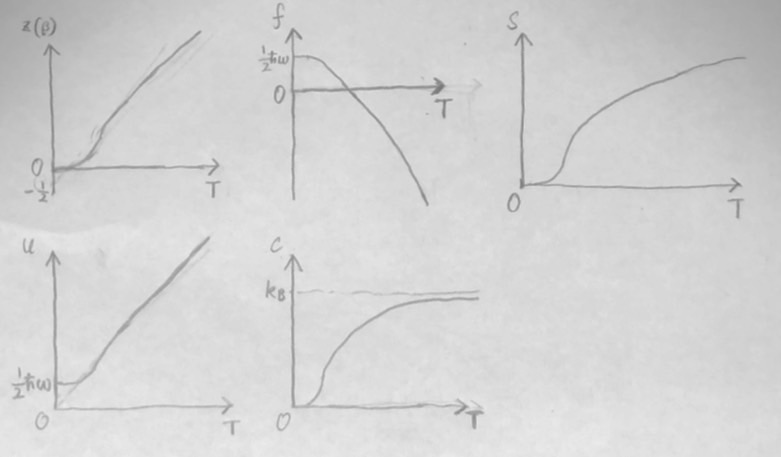
\includegraphics[height=8cm]{oscillator_system.jpg}
    \caption{振動子系におけるそれぞれの熱力学量の温度 $T$ に関するグラフ}
    \label{fig:oscillator}
  \end{center}
\end{figure}

\section{固体の比熱の Einstein 模型}
\begin{itembox}[l]{Q 16-5.}
  独立な調和振動子の集まりの系として記述される系 $X$ において$\dd{\omega}$ が十分小さいとして、角振動数が $\omega$ から $\omega + \dd{\omega}$ の範囲にある調和振動子の個数を $g(\omega)\dd{\omega}$ と定義する。つまり $g(\omega)$ は調和振動子の角振動数の個数分布関数である。
\end{itembox}
このとき角運動量が $\omega$ である調和振動子 1 個の Helmholtz 自由エネルギー, エントロピー, 内部エネルギー, 比熱をそれぞれ $f(\omega), s(\omega), u(\omega), c(\omega)$ と書くこととすると、$\dd{\omega}$ が十分小さいことから近い角運動量の変数を個数倍して積分することで元の変数と一致する。これより次のような式が成り立つ。
\begin{align}
  F & = \int_0^\infty\dd{\omega}g(\omega)f(\omega) \\
  S & = \int_0^\infty\dd{\omega}g(\omega)s(\omega) \\
  U & = \int_0^\infty\dd{\omega}g(\omega)u(\omega) \\
  C & = \int_0^\infty\dd{\omega}g(\omega)c(\omega)
\end{align}

\begin{itembox}[l]{Q 16-6.}
  ある元素の原子 $n$ [\si{mol}] からなる個体を考える。Einstein 模型では、結晶を構成するそれぞれの原子は平衡位置の回りに独立に同一の角振動数 $\omega_E$ を持って調和振動すると考える。ここで次の観測結果に対して Einstein 模型は妥当性があることを説明せよ。
  \begin{enumerate}
    \item (高温での固体の比熱の振る舞い : Dulong-Petit の法則) 十分に高温では、$n$ [\si{mol}] の固体の比熱 $C$ は、固体を構成する物質によらずに、$3nR$ の一定値を取る。ここで、$R = 8.314\ldots$ [\si{J/(mol\cdot K)}] は気体定数である。
    \item (低温での固体の比熱の大雑把な振る舞い) 温度 $T$ が $0$ に近付くとき、固体の比熱 $C$ は小さくなっていく。温度 $T$ が $0$ に近付く極限では、比熱 $C$ はゼロになるようだ。
  \end{enumerate}
\end{itembox}
調和振動子の角振動数の個数について、各原子の自由度が $3$ であるから Avogadro 数 $N_A = 6.02\ldots\times 10^{23}$ [\si{1/mol}] を用いて全体の個数は $3N = 3nN_A$ であることが分かる。
これより Einstein 模型における調和振動子の角振動数の個数分布関数 $g(\omega)$ は次のように表される。
\begin{align}
  g(\omega) = 3N\delta(\omega - \omega_E).
\end{align}

これより比熱は次のように表される。
\begin{align}
  C & = \int_0^\infty\dd{\omega}g(\omega)c(\omega)                                            \\
    & = \int_0^\infty\dd{\omega}3N\delta(\omega - \omega_E)c(\omega)                          \\
    & = 3Nc(\omega_E)                                                                         \\
    & = 3Nk_B\qty(\frac{\frac{1}{2}\beta\hbar\omega_E}{\sinh\frac{1}{2}\beta\hbar\omega_E})^2
\end{align}
高温の漸近領域において比熱 $C$ は次のようになる。
\begin{align}
  C & = 3Nk_B\qty(\frac{\frac{1}{2}\beta\hbar\omega_E}{\sinh\frac{1}{2}\beta\hbar\omega_E})^2 \\
    & \approx 3Nk_B\qty(1 - \frac{1}{12}\qty(\frac{\hbar\omega}{k_BT})^2 + \cdots)            \\
    & \approx 3nR
\end{align}
低温の漸近領域において比熱 $C$ は次のようになる。
\begin{align}
  C & = 3Nk_B\qty(\frac{\frac{1}{2}\beta\hbar\omega_E}{\sinh\frac{1}{2}\beta\hbar\omega_E})^2 \\
    & \approx 3Nk_B\qty(\frac{\hbar\omega}{k_BT})^2e^{-\frac{\hbar\omega}{k_BT}}              \\
    & \approx 3nR\qty(\frac{\hbar\omega}{k_BT})^2e^{-\frac{\hbar\omega}{k_BT}}
\end{align}
よって低温領域で温度 $T$ が小さくなっていくとき、比熱 $C$ が小さくなる。
\begin{align}
  \lim_{T\to 0} C & = \lim_{T\to 0}3nR\qty(\frac{\hbar\omega}{k_BT})^2e^{-\frac{\hbar\omega}{k_BT}} = 0.
\end{align}
これらの結果は観測結果と一致している為、妥当性がある。

\begin{itembox}[l]{Q 16-7.}
  固体の比熱の Einstein 模型は次の実験事実と合致しないことを確認せよ。
  \begin{enumerate}
    \item (低温での固体の比熱の精密な振る舞い) 温度 $T$ が $0$ に近付くとき、固体の比熱 $C$ は $C \propto T^3$ であり、$\lim_{T\to 0} C = 0$ となる。
  \end{enumerate}
\end{itembox}
低温領域で温度 $T$ が小さくなっていくとき、比熱 $C$ は次のように小さくなる。
\begin{align}
  C & \approx 3nR\qty(\frac{\hbar\omega}{k_BT})^2e^{-\frac{\hbar\omega}{k_BT}} \\
    & \propto \frac{1}{T^{2}e^{\frac{1}{T}}}
\end{align}
これより $C \propto T^3$ とはならない為、固体の比熱の Einstein 模型は実験事実と合致しない。


\end{document}
